\newpage
\section{有機ELディスプレイを使ってみよう}
有機ELディスプレイをHSPで使ってみましょう。I2Cに有機ELディスプレイ(\#214)をつないでみましょう。HSPスクリプトエディタで\textasciitilde /05/oled.hspを開いて実行してください。
  \begin{minipage}[t]{0.3\columnwidth}
    \begin{figure}[H]
      \centering
 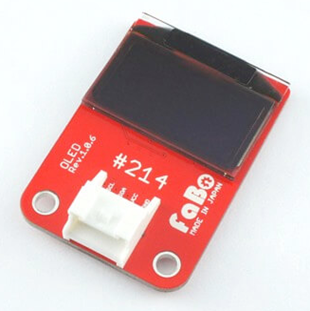
\includegraphics[width=\linewidth]{images/chap05/text05-img032.png}
    \caption{有機ELディスプレイ}
  \end{figure}
\end{minipage}
  %\hspace{0.01\columnwidth} % ここで隙間作成
  \begin{minipage}[t]{0.5\columnwidth}
    \begin{figure}[H]
      \centering
    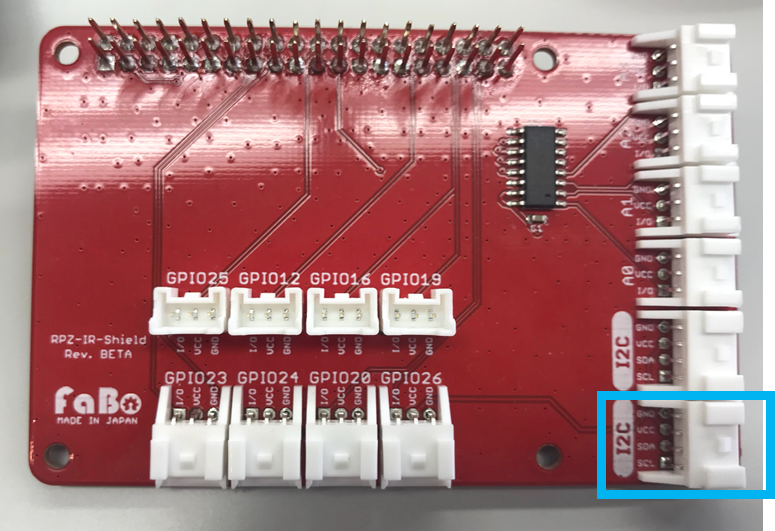
\includegraphics[width=\linewidth]{images/chap05/text05-img033.png}
    \caption{I2C}
  \end{figure}
\end{minipage}

\begin{lstlisting}[caption=oled.hsp,label=oled.hsp]
#include "hsp3dish.as"
#include "rpz-gpio.as"

redraw 0
font "",20
pos 20,20
mes "有機ELディスプレイを見てね\nカンマ(,)で改行するよ"
redraw 1

oled "Good Morning,Good Bye,Good Afternoon"
<#blue#;ELディスプレイに#>
<#blue#;Good Morning#>
<#blue#;Good Bye#>
<#blue#;Good Afternoon#>
<#blue#;と表示します。#>

wait 100
\end{lstlisting}

有機ELディスプレイに文字を表示するには\code{oled}命令を使います。
\code{oled “表示したい文字”}と使います。英語か記号を表示することができます。日本語は表示できません。,(カンマ)を使って、改行することができます。\\

\begin{tcolorbox}[title=\useOmetoi]
\begin{enumerate}
\addex{自分の名前(アルファベット)を有機ELディスプレイ(\#214)に表示してみましょう。}
\addex{自分の名前の下に、\ruby{隣}{となり}の人の名前(アルファベット)を有機ELディスプレイ(\#214)に表示してみましょう。}
\end{enumerate}
\end{tcolorbox}
